\documentclass[type=bachelor]{thuthesis}
\usepackage{thuthesis}
\usepackage[section,newfloat=true]{minted}
\usepackage{hypcap}
\usepackage{etoolbox}
\usepackage{setspace}

% fix minted fontsize and linespacing
\AtBeginEnvironment{minted}{\singlespacing%
  \fontsize{10}{10}\selectfont}
% add frame
\setminted{frame=lines,framesep=2mm}
% code env to support page break
\newenvironment{code}{\captionsetup{type=listing}}{}

% 中文字体设置
\setCJKmainfont{Noto Serif CJK SC}[AutoFakeSlant=true]
\setCJKsansfont{Noto Sans CJK SC}[AutoFakeSlant=true]
\setCJKmonofont{Noto Sans Mono CJK SC}[AutoFakeSlant=true]

\graphicspath{{figures/}}

\ctexset{
  chapter = {
    name = {},
    number = \arabic{chapter}
  }
}

\geometry{margin=25mm}

\begin{document}

\frontmatter
\thusetup{
  ctitle={EdenApple - Lisp 解释器},
  etitle={EdenApple - a Lisp Interpreter},
  cauthor={刘宇辉},
  cdegree={学士学位},
  cdepartment={计算机与信息工程},
  cmajor={软件工程},
  csupervisor={曹芝兰},
  ckeywords={解释器, scheme, lisp},
  ekeywords={interpreter, scheme, lisp}
}

\begin{cabstract}
编程语言是现如今计算机系统中的核心,无论何种计算机系统基本上都通过某一个或几个编程语言来编写组织功能。而关于编程语言与编译器的研究也一直都是计算机研究中非常重要的一部分。编程语言与编译器和解释器的实现是两个相互联系密切却又有些相互独立的部分。编程语言的特性是程序设计最直接依赖的规则,而语言特性的实现离不开编译器与解释器提供的一些特定的功能。当今编译器的前后端架构为这种分离提供了一种统一的框架,更是为编程语言与编译器的研究建立了坚实的基础。本文探索动态类型语言的解释器实现方式以及优化方案。

本文尝试通过完成一个较为完整的解释器来探索类似scheme的动态类型语言的解释器的必要组成部分以及在解释器实现中可能的优化方案。首先探讨了动态语言需要的几个基本语言特性,随后在实现中尝试提供这些语言特性所需要的基础功能,并在此过程中探讨语言特性所带来的各种实现与优化上的限制。

论文最终提供了一个完整的简化lisp语言的解释器实现,提供了词法作用域,call/cc,尾递归优化,递归数据定义的特性。
\end{cabstract}

\begin{eabstract}
Programming language is the core of today's computer system. Almost every sophisticated computer system is built up on one or several computer languages. The research about lanuage and compiler and interpreter is one of the most important parts of research in computer science. The two fields are closely related but developed independently. Modern compiler infrastructure are divided into frontend and backend, which established solid basis for the development of language and compiler and interpreter. In this paper we'll explore the implementation and possible enhancements of the interpreter of dynamic type languages.

In this paper, we'll explore the vital components and possible enhancements in dynamic type languages like scheme by implementing a function complete interpreter. First, a few language features are discussed. And then implementation details include basic features needed, restrictions and enhancements are explored by implementing them.

Finally, there is a feature complete interpreter for a small lisp language. The core language features it provides are lexical scoping, call/cc, tail call optimization and mutually recursive data.
\end{eabstract}

\makecover

\mainmatter
%% page style
\fancypagestyle{hubu@thesis}{%
  \fancyhead[R]{\xiaowu\textsl{湖北大学本科毕业论文(设计)}}
  \fancyfoot[C]{\xiaowu\thepage}
  \renewcommand{\headrulewidth}{0pt}
  \renewcommand{\footrulewidth}{0pt}}
\pagestyle{hubu@thesis}

\xiaosi
%
% 第一章 简介
%
{
    \let\centering\raggedright
    \chapter*{绪论}
}
\addcontentsline{toc}{chapter}{\hspace{1em} 绪论}
\label{ch:intro}
\thispagestyle{hubu@thesis}

在本论文中,通过实现一个精简的Lisp解释器,研究如何实现Lisp这种动态类型函数式编程语言的运行时。论文首先探索了一个解释器的基本结构,再以几个基本的语言特性为目标探索了编程语言的运行时中的两种基本上下文,并且以最终实现一个可以运行的解释器来深入探索编程语言的运行行为。

编程语言的研究是计算机发展史上一个一直不曾停歇的主题,从最早期的指令输入,到汇编语言,到具有过程抽象的B语言,C语言,在到面向对象,函数式,多范式编程语言,以及具有复杂类型系统的Haskell,和用于定理证明的Coq,Idris等。编程语言从最早期的被忽视,到功能单一的抽象,如今已发展到百花齐放的时代。

现代的编程语言已经不再是一个可以简单的定义其功能的概念,作为具有一类形态的抽象工具,编程语言的内涵已经跨越逻辑学,科学计算,工程应用等多门学科。在当今社会,编程语言可以称之为社会基石的基石。

对于一个编程语言,程序如何定义,如何运行是一个基本的问题,而解答这个问题可以通过解释器这种抽象模型。一个解释器是运行一段计算机程序并计算得到最终结果的程序。研究编程语言的一个方向便是如何实现一个能够支持特定语言特性的解释器。

Lisp作为一个编程语言,可以看作是Lambda Calculus\cite{Church1932A}理论的一个直接翻译。Lambda Calculus是现代大多数函数式编程语言的理论基础,是与图灵机等价但在某些方面甚至比图灵机更加意义重大的一个理论。Lisp 由人工智能之父John McCarthy发明,并于1960年发表于ACM\cite{mccarthy60}。Lisp现在通常表示函数式编程语言中的一个族系,常见的Lisp系语言有Common Lisp, Scheme\cite{sussman1998scheme}, ELisp\cite{Lewis1993elisp}, Clojure\cite{hickey2008clj}。Lisp以S-Exp作为语法规则,因此带来的宏(Macro)功能能够让代码本身如同数据一样被操作。Lisp对后世许多编程语言造成了深刻影响。比如现今通用的词法作用域,垃圾回收机制,JS与Python中的闭包,等等。Lisp可以看作是编程语言发展历史中一个富有生命力,经久不衰的分支。

初代Lisp的具体内容可以参考\textit{LISP 1.5 programmer's manual}\cite{lisp1.5}。在该手册中详细讲述了Lisp的形式化定义,以及Lisp的语义与数据如何以S-Exp表达。

不同于解释执行。相对于编译器将一个编程语言转换为令一种语言,通常是线性的机器指令序列,解释执行通过一段现有的程序解析程序的语义结构并计算输入程序的结果。而无论是编译器还是解释执行,核心的一点便是对编程语言本身的解释,编译器只有在知道如何解释编程语言之后,才能够将对应的行为以另一种语言表达。而在本论文中,探索的便是这种解释的行为,具体的,采用了一种编译与解释执行相结合的解释流程。

对程序的解释当然离不开程序本身,因此,本论文虽然探索的是解释器的实现,但却离不开具体的语言特性,解释器的行为便是对具有这些语言特性的程序的解释。

在本论文中,所研究的解释器以Lisp作为具体语言,以闭包,call/cc,尾调用优化三个语言特性为目标,能够运行具备上述特性的Lisp程序。

\section*{国内外研究现状}

本论文研究的是Lisp语言的解释器,首先,Lisp语言本身用途广泛。Lisp在早期的AI相关研究中扮演重要的角色,事实上,正是因为AI领域的研究,Lisp才得以发明。Lisp因为本身结构简单,组合灵活,在教育上常用作一种教学用语言,同时,在工业上也有相当广泛的应用。曾应用于NASA。硅谷创业之父Paul Graham在他的《黑客与画家》中也描述了他创业时使用Lisp快速搭建出业务系统并因此击败竞争对手的故事。

Lisp方言以及对应方言解释器的探索一直不曾终止。上个世纪便有着Common Lisp,ELisp,scheme等各具特色的流行变体。在近些年,亦有Lisp的变体出现,比如Clojure,Clojure作为一个新兴的Lisp系方言,在国内外也有着越来越多的使用案例。在国内有着LeanCloud, 一熊科技, 火币网等创业公司以Clojure作为主要开发语言。同时Clojure的JS版本ClojureScript也渐渐的在前端圈火热起来。

在通信等需要高可靠特性的环境下,通常使用Erlang\cite{armstrong07}来作为基础设施。而基于Erlang虚拟机的Erlang变体Elixir也深受Lisp的影响。同样受到Lisp影响的还有Julia,R,SPSS等。

Racket\cite{plt-tr2010-ref}项目是一个scheme的超集,由多个大学与企业主导,在其主页中,将Racket描述成是一个新语言特性的研究场。这表明在现阶段,在有关语言特性的研究中,Lisp仍然占据一定的分量,与Haskell,Ocaml等语言都是语言研究中的主要工具。

可以看到Lisp(包括其灵活的文法,完善的基本语言特性)可以看作是语言研究的一个非常完备的原型,在其上可以方便的演变出各种语言特性。

除了Lisp系语言的发展以外,现阶段编程语言的研究一个是工程应用上追求效率与正确性的努力,这方面成就有近些年的Swift,Rust等,也有走向完善类型系统的方向的Haskell系,ML系语言。而每一个方向的研究都离不开对语言运行环境的设计以使其能够高效运行。可以说,这些语言的大部分研究重点在于运行环境,或者说是``解释器''的设计。

在这方面的成果有LLVM(一个编译器框架),G-Machine(一个函数式语言的运行环境)等等。

\section*{研究内容}
%\addcontentsline{toc}{section}{研究内容}

本论文研究如何实现一个具备词法作用域,call/cc,尾调用优化这三种基本语言特性的基础Lisp解释器以及该语言运行时的模型。为讨论方便,将其命名为EdenApple,以表示其与其他解释器或编译器的区别。EdenApple采用scheme作为参考语言。

在此选择Lisp作为解释器实现的目标语言一个是因为Lisp族系语言本身在语法特性上高度统一并且丰富,其次,Lisp的文法(S Expression)也以其简单强大的表达能力闻名,这使得研究过程中可以专注于语言特性本身。

Lisp的语法特性灵活,导致Lisp解释器或者编译器的实现往往异常困难。半个世纪以来有过许许多多的尝试去实现一个高效的Lisp运行环境。而这其中的关键,便是如何设计一个高效的运行时模型同时完整的支持Lisp的语义。

这些尝试带来了各种不同的Lisp实现,比如T语言以及其Orbit编译器\cite{Adams1986ORBIT},Chez Scheme\cite{dybvig2006chez},等等,他们在运行机制,编译目标,运行效率等等方面各有千秋。本论文中的解释器由reader和VM组成,是一种基于堆的解释器模型。而对其实现,虽然不限置于任何语言,本论文选择JavaScript作为运行的宿主环境。

EdenApple的意义在于探索如何实现一个完整的程序运行模型,因此,在本论文中,讨论的侧重点在于解释器的VM的结构以及运行原理。VM的结构主要基于Kent. R Dybvig的\textit{Three implementation models for scheme\cite{dybvig87timpl}},其中letrec的实现主要参考Kent的另一篇文章\textit{Fixing letrec\cite{Waddell2005Dybvig}}。

\section*{论文组织}
%\addcontentsline{toc}{section}{论文组织}

本论文主要分为两部分,前半部分讨论语言特性与解释器结构,后半部分讨论EdenApple的实现。

在\nameref{ch:lang features}中讨论EdenApple的三个基本语法特性,在\nameref{ch:interp structure}中描述解释器的基本结构,随后在\nameref{ch:parser}中讨论如何实现解释器的解析器部分,解析器的实现采用了parser combinator技术。最后在\nameref{ch:vm impl}中详细讨论EdenApple的虚拟机模型以及该模型如何支持语言的运行,具体的,如何实现上述的三个基本语言特性。
%
% 第二章 语言特性
%

\chapter{常见语法特性}

Lisp经过半个多世纪的发展,产生了许许多多的方言,这些方言不仅逐渐完善了Lisp最初的核心功能,还将许多思想带入到了Lisp系语言。比如hygienic macro,lexical scoping,first class continuation,等等。接下来简单讲解下lexical scoping,first class continuation与proper tail call optimization。

为了方便描述,本论文接下来将以scheme作为主要描述对象,scheme是Lisp的一个方言。是众多Lisp方言中较为简洁明了的一个方言,同时仍然具备完整灵活的主要语言特性。关于scheme以及其实现的更多资料,可以参考Kent Dybvig的The Scheme Programming Language\cite{dybvig09scm},SICP\cite{sicp},Lisp in Small Pieces\cite{que03}等书。

\section{词法作用域}

lexical scoping是词法作用域的意思,也就是当程序需要查找一个变量的时候,会以代码中的词法结构为依据查找。这种查找策略广泛应用于现代的各个语言中,而且符合人的直觉。以至于很难去理解若不是词法作用域还能存在怎样的查找策略。所以在此先提及动态作用域然后给出例子对比两种不同策略下行为的差异。

一种动态作用域的查找策略是自上而下搜索程序当前运行状态中的控制栈,也称为调用栈。这就需要该语言具备子过程或者称为函数的抽象。函数在程序运行过程中可以相互调用,每一次调用都会为该函数维护一个临时的数据区,存放本地变量,传入参数,返回地址等信息。这种数据区叫做调用帧,由于函数调用天然具备先进先出的特征,这些调用帧通常以栈的方式组织。动态作用域的变量解析便可以沿着这条调用帧链自顶向下查找对应名字的值。

还有一种动态作用域的模型是将所有变量放入到一个空间中。

而词法作用域对于变量的解析严格限制于变量解析在代码中的位置,沿着代码中的词法结构所构造出的作用域链查找。

比如在这段C代码中:

\begin{code}
\begin{minted}{C}
int hello = 1;

int fun() {
  return hello;
}

void call() {
  int hello = 2;
  int result = fun();
}
\end{minted}
\caption{作用域示例代码}
\end{code}

变量hello有两处定义,一处在全局,定义为1,一处为call函数的本地变量,初始化为2。fun函数调用的结果毫无疑问是1。按照词法作用域,fun在获取hello的值时,会在定义处,也就是fun函数所创建的作用域,以及该作用域的上级词法作用域(这里只有一个全局)去解析hello变量的值。

如果把该示例的全部内容看作是全局作用域,可以发现,fun的定义在代码文本结构上是全局中的一部分,所以fun所构建的作用域以全局作为上级作用域,而对hello变量的引用是发生在fun的定义中的,自然对hello的解析也是从fun所创建的作用域开始。这便是词法作用域中词法一词的由来。

与此相对应的,如果采用动态作用域,hello的解析会依赖于程序运行时的调用栈一级一级向上查找变量。那么此时结果应该为2。

由于动态作用域的违反直觉的行为,编程语言往往以词法作用域为主。然而也有某些语言采用该策略,比如perl,elisp等。动态作用域的一个优点是配置的注入变得非常直接,而且动态作用域在实现上往往也非常直接简单。因为不需要单独维护一个变量解析的环境,程序执行时的控制栈就是变量解析的环境。

\section{call/cc}

call/cc是scheme中的一个语法式。通过call/cc,scheme提供了first class continuation的特性,也就是可以将continuation作为值传递。这里continuation的含义是程序接下来要执行的事情。往往,对于一个程序的执行过程,可以将其抽象成当前的计算和接下来需要执行的事情,而程序的运行可以表示为将当前的计算结果传入下一个continuation。

下面以一段实际的scheme代码为例:

\begin{code}
\begin{minted}{scheme}
(define k)

(let ([x (call/cc
          (lambda (return)
            (set! k return)
            0))])
  (display x))

(k 1)
(k 2)
(k 3)
;; => 0123
\end{minted}
\caption{call/cc示例}
\label{call/cc sample}
\end{code}

程序\ref{call/cc sample}中我们首先定义了变量k,接下来这段的语义是调用call/cc并将结果保存到x,然后打印x。在call/cc中的$\lambda$函数中将传入的return保存到了k变量。之后分别以1,2,3调用k。

在这里让人感到有意思的是调用k的含义。通过输出我们看到display语句被执行了四遍,其中的0是正常的执行流程,后面的123显然是调用k所得的结果,但是k的值显然并不是一个函数抽象,display也并不属于任何一个函数抽象。

这正是first class continuation带来的效果。每一次k的调用都会将整个程序的执行状态恢复到call/cc调用刚结束的时候。而call/cc调用结束之后的事情包括将结果绑定到x并打印x。这里可以将k看作是一个只能回到某一特定时间节点的时光机。

这个特性以及其变体在其他语言,比如SML,OCaml,Haskell中也有相应的实现。通过call/cc可以实现许多复杂的控制结构,比如McCarthy的amb操作符\cite{mccarthy61},coroutine,异常处理,线程,等等。

\section{尾调用优化}

在程序执行过程中一个基本的操作便是函数调用,通常伴随着函数调用操作,控制栈上会压入一帧来保存本次调用需要的数据,或者类似的行为。但是,随着函数调用深度的加深,尤其是在递归调用中,控制栈的大小会越来越大,直到超过一定限制导致程序错误。这里介绍一种特殊的递归情况,在这种情况下的递归调用不需要增长控制栈的大小,由此可以带来无限递归的可能。

在一个函数的具体执行流程中,当某一个函数调用操作的直接后继操作是返回(return)时,该操作可以被称之为尾调用(tail call)。尾调用具有如下特性:

\begin{enumerate}[1.]
\item 是一次函数调用的一部分,而不是全局中的一条语句
\item 尾调用的结果为当前函数的结果
\end{enumerate}

比如下面的示例中的所有t函数的调用。

\begin{code}
\begin{minted}{scheme}
(define (t i)
  (display i)
  (+ i 1))

(lambda ()
  (t 1))

(lambda ()
  (let ([x 3])
    (t x)))

(lambda ()
  (let ([x 3])
    (if (> x 2)
        (t x)
        (t (- x 1)))))
\end{minted}
\caption{尾调用示例}
\end{code}

需要注意的是尾调用并不仅仅指符合上述要求的自递归或互递归,任何符合上述条件的尾调用都是尾调用。但是尾调用使得符合条件的线性递归调用不再担心控制栈溢出的情况,详细内容可以参考SICP\cite{sicp}的1.2.1节和5.4节。

除了scheme等函数式语言之外,尾调用在微软的CLR,下一版本的JS中都有相应的实现。
%
% ch03 解释器
% 讲解Lisp解释器的组成部分。
%

{
    \let\centering\raggedright
    \chapter{解释器结构}
    \label{ch:interp structure}
}    \thispagestyle{hubu@thesis}


本章节讨论一般Lisp解释器的结构,相关的技术以及EdenApple这个解释器实现的具体结构。EdenApple的VM与Compiler主要参考R. Kent Dybvig的Three implementation models for scheme\cite{dybvig87timpl}中的Heap-based model。语义上的细节主要参考scheme语言规范r6rs\cite{r6rs}。

解释器的工作原理在\textit{Essentials of Programming Language\cite{friedman2001eopl}}中有很好的描述,本论文的实现亦有沿用其中的思路。

EdenApple的基本结构如图\ref{fig:interp structure}所示:

\begin{figure}[h]
\begin{center}
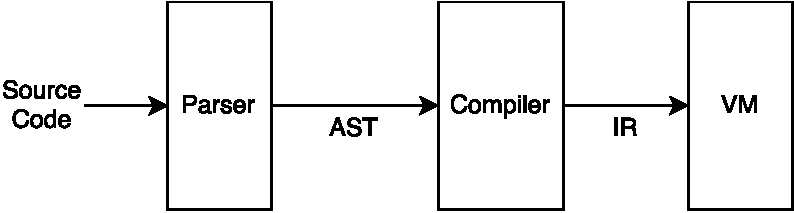
\includegraphics[width=\textwidth]{interpreter}
\end{center}
\caption{解释器结构}
\label{fig:interp structure}
\end{figure}

Lisp以及Scheme虽然是动态类型语言,但是语言的运行环境的实现方式上却是多种多样的。通常动态语言是解释执行的,scheme虽然也有许多实现是解释执行的,但是大多数都采取先编译后执行的策略。除了解释执行与编译执行之外,也有将scheme代码编译成C代码的实现,比如chicken。

与C,Java等语言不同的是,一些scheme实现虽然先编译后执行,但是编译的过程是隐含的,而非显式的。也就是scheme运行环境的输入是scheme源代码,而输出便直接是结果。在内部,源代码先编译成,或递增式编译成虚拟机字节码或者机器码,然后执行。

除了compiler和VM或者RTS(Runtime System)部分,一个解释器另一个重要的组成部分是reader,reader负责两个功能,对源代码进行parse,展开所有的宏,完成后一项功能的组件通常叫做expander。expander的功能自成一套体系,超出本论文的范围,故EdenApple的实现中不带有expander。

下面分别描述reader,compiler,VM。

由于EdenApple的实现重点在于如何构建一个运行最小Lisp的VM,compiler的功能比较单一,仅仅是对AST进行转换,翻译成VM能运行的代码块,没有进行更多的优化pass。因此本论文接下来的内容将着重与parser的构建以及VM的实现。

\section{reader}

虽然EdenApple不会带有expander功能,但是Lisp语言的macro功能是非常强大的,所以在此介绍下Lisp的macro功能。

在绪论\ref{ch:intro}中提及Lisp中的代码以及数据具有同构性(homo-iconic)。即代码即数据,代码可以像数据一样被操作,被变换,而这种变换便是通过macro来实现的。

在C中也有宏,但是C中的宏是基于文本替换的,而在scheme中,宏所操作的对象是Lisp中的基本数据,是代码本身的数据表示,因此会带上代码本身的类型信息,层次结构。而与之相对应的,C中的宏所操作的文本对于代码本身的结构与类型信息一无所知。因此scheme宏能够以更简单的方式实现更多的功能。下面是一个scheme中的宏:swap!,交换两个变量的值。

\begin{code}
\begin{minted}{scheme}
(define-syntax swap!
  (syntax-rules ()
    ((_ a b)
     (let ([tmp a])
       (set! a b)
       (set! b tmp)))))

(let ([c 1]
      [d 2])
  (display c)(display d)
  (swap! c d)
  (display c)(display d))

;; => 1221

;; (swap! c d) 
;; 将会在运行前被替换为
;; (let ([tmp c])
;;  (set! c d)
;;  (set! d tmp))
\end{minted}
\caption{macro示例}
\label{listing:macro-sample}
\end{code}

在\ref{listing:macro-sample}中,syntax-rules创建了一个变换规则,可以看到变换的过程是将模板中的a,b替换为宏调用时传入的c,d。这里syntax-rules是一个比较高阶的宏系统。这种宏格式规整,通过模式匹配与模板相结合的方法对代码进行转换,相当于是拥有自己的一套语言。在scheme中也有syntax-case这种比较底层的宏系统可以使用scheme代码本身对scheme代码进行转化。

有关scheme中宏的更多内容可以参考The Scheme Programming Language\cite{dybvig09scm}的第八章。

在expander步骤之前,reader的另一功能是将源代码解析成AST(抽象语法树)。parser与具体的程序功能几乎没有关系,但仍然是一个完整的解释器必不可少的一部分,在这里,EdenApple采用parser combinator的方式编写parser部分。

\section{compiler}

compiler负责将完成解析之后的AST转换为目标机器的指令序列(可能是机器码,也可能是VM的字节码)。

一种常见的compiler结构由前后端组成,前端负责将语言转换优化到中间表示,后端负责针对具体机器目标对中间表示进行优化并进行后续的register selection和codegen步骤。

但是在EdenApple中,compiler的作用被弱化,这里所采用的编译只是简单的将scheme的语法元素按序直接翻译成VM指令。因为此处的VM是专为Lisp语言设计,大部分的上下文管理工作,都直接依托于VM来管理,所以在语言语义与VM指令之间并不存在过大的间隔。因此这种直接翻译的做法是可行的。

\section{VM}

VM是程序能够运行的核心。通常一个机器能够运行体现在他能够不断的接收指令并根据指令将机器从当前状态迁移到下一个状态。这种机器状态的不断变换即一个机器运行的表现。这些机器的状态可以有多种表现方式,常见的便是寄存器,内存等等。

现代编程语言所编写的程序在运行时往往需要维护程序执行时的许多内部状态以支持这些编程语言所提供的抽象。比如函数的抽象以及函数调用需要的调用栈,变量的维护。本论文的VM设计便是主要围绕如何管理这些内部状态这个问题。

由此引申出上下文(context)的概念。管理程序运行时所需变量的存储与索引的相关结构,我们称之为环境(Environment)。除了环境以外,程序运行一般还需要一个控制上下文(Control Context)。通常编程语言都会有函数这种抽象,函数的调用隐含着停下当前的动作,前往执行另一个动作并在完成之后回到当前的动作这样一个行为,这种回到的操作,也就是return操作,是在运行时决定的,一个函数在执行完成之后需要回到哪一个地方是有程序运行时的函数调用情况决定的,在何地被调用,便回到何地。显然,需要一种结构来管理这种运行时的信息,这便是控制上下文。

在C语言中,因为无法在函数中定义函数,因此按照词法作用域,一个变量要么是当前函数的本地变量,要么是全局变量,而其中的本地变量只有在函数执行期间有效而且每次调用的本地变量与其他调用互不相关。可以看到,本地变量的生命周期与函数调用帧完全符合。所以在这种情况下,函数调用栈,也就是C的控制上下文中每一帧额外存储函数的本地变量。在这一点上,C中的环境与控制上下文有一部分的交叉。

而在JS,scheme等动态语言中,允许在函数中定义函数,按照词法作用域,这些函数将隐含关联定义处的环境。所以存在一种情况,一个函数执行完成后,他的本地变量仍然需要能够被访问,如下面代码所示:

\begin{code}
\begin{minted}{scheme}
(define (mk-closure i)
  (lambda ()
    (set! i (+ i 1))
    i))
(define inc-and-get (mk-closure 0))
(inc-and-get) ;; => 1
(inc-and-get) ;; => 2
(inc-and-get) ;; => 3
\end{minted}
\caption{闭包示例}
\label{listing:closure-sample}
\end{code}

在\ref{listing:closure-sample}中,mk-closure的调用结束后返回了在mk-closure中定义的一个lambda函数,而该lambda函数引用了mk-closure的参数i。在后续的inc-and-get调用中,自增了i的值并返回。

此时函数抽象表达式的值通常称之为闭包(closure),以示他与一般意义上的函数存在的一些区别,可以将closure看作是有函数本身以及函数定义时所在的环境组成的二元组。

所以在语言具备闭包特性的情况下,环境与控制上下文难以如同C语言中那样简单直接的组合在一起。但是并不是表示只能够将两个上下文完全分开管理,因为栈式结构中本地变量的管理与访问速度相比较于放入堆中的情况更加简单而且快速,所以也存在过相关的研究与结果,详情参考\textit{An introduction to Scheme and its Implementation\cite{wilson96intro}}, \textit{Three implementation models for scheme\cite{dybvig87timpl}}以及chez scheme。 

关于闭包在内存中的结构,可以参考图\ref{fig:closure-mem-layout}:

\begin{figure}
\centering
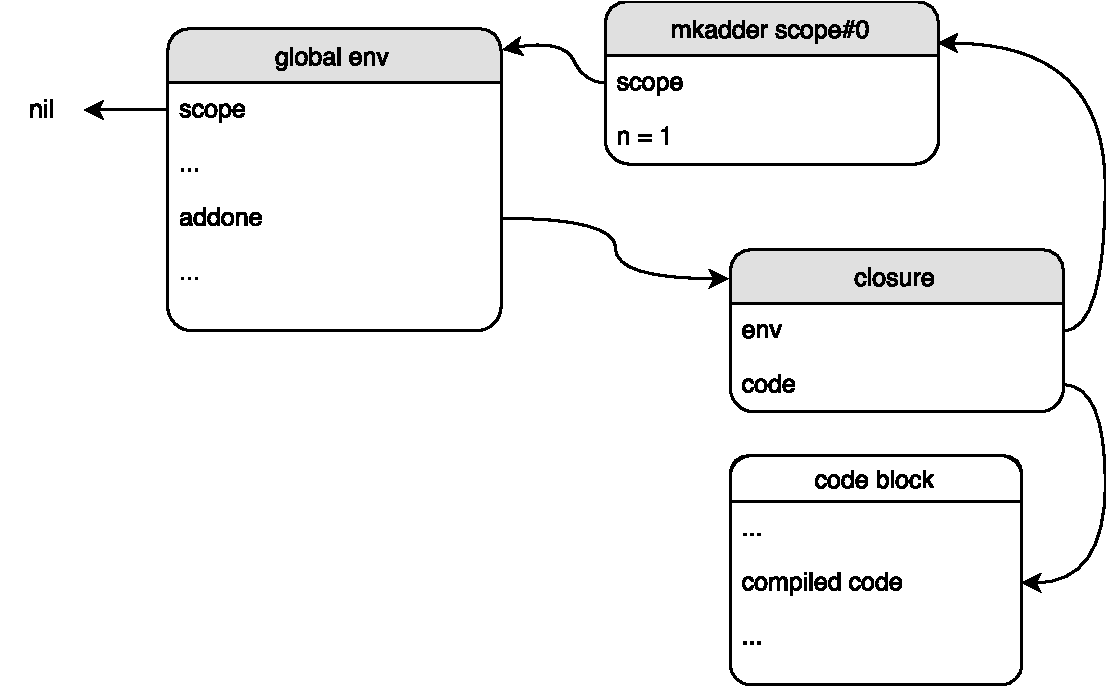
\includegraphics[width=300pt]{closure-sample.pdf}
\caption{闭包内存布局示例}
\label{fig:closure-mem-layout}
\end{figure}

在本节中,主要讨论了程序运行需要的两种上下文,而这也是EdenApple的VM所要维护的核心结构,在第\ref{ch:vm impl}章中将详细地描述如何实现VM。
%
% 第4章 parser
% 这个章节讲monad和parsec
% 毕竟monad也算是程序运行的一种抽象,还是有必要讲一讲的,
% 顺便把上次写的monad和parser的一点感想直接丢过来。
% 凑凑字数 <- 真实目的
%

% haskell中运算符的定义

\newcommand{\hsbind}[0]{$>\!\!>\!\!=$}
\newcommand{\hschoice}[0]{$<\!\!|\!\!>$}

\chapter{Monadic Parser Combinator}

对于一个完整的解释器而言,parser是必不可少的一部分。在上一章节中提及过EdenApple中的reader的唯一功能即parser。

通常,一个parser可以通过手写状态机,或者使用parser generator来生成,在这里,将描述一种以函数组合的形式来完成parse的方法,称之为parser combinator。

parser combinator作为一种parser编写的技巧并不怎么常见,这种技巧常见于函数式编程语言中,是一种将parser看作为函数并通过各种组合子一步步构建出复杂的解析规则的做法。一个比较出名的parser combinator的应用是Haskell中的parsec\cite{leijen01parsec}。

或许是因为函数式编程语言比较小众,而且parser combinator在处理左文法以及在复杂文法和性能上的缺点等等原因,在现实应用中,parser combinator不怎么流行。当然,在对parser combinator的研究上也一直不曾停歇。

\section{parser函数}

首先,从功能上来看,parser所完成的工作可以描述为,给定一个字符串,按照语言特定的语法规则解析这个字符串,最终返回一个解释结果,这个结果通常是一个树状结构的数据,反映了对应语法规则下的一个具体的语义结构。

如果将函数的定义与parser的工作过程对比,可以发现,一个parser可以看作是一个接收字符串为参数,返回一个解释结果的函数。

但是,仅仅是这种将parser看作是函数的看法并不能够带来什么实质性的去构建一个parser的方法。

在函数式编程中,一个重要的概念是高阶函数,一个函数可以接收函数作为参数,也可以返回一个函数。也就是说可以定义一类操作,将多个操作组合拼接成一个新的操作。parser combinator之所以称之为parser combinator,即是因为他的思想是将子parser按规则组合成为所需要的parser。

\section{组合子}

在描述组合子之前,先给出一些文法的例子以观察文法定义本身的组合特性。

首先,给出一个最简单的文法的例子:

\begin{listing}
\begin{verbatim}
<sample> ::= <chara><charb>
<chara>  ::= a
<charb>  ::= b
\end{verbatim}
\caption{顺序结构文法定义示例}
\label{lst:seq-syntax-sample}
\end{listing}

在\ref{lst:seq-syntax-sample}中,sample的定义由chara和charb两个自定义组成,解析sample的过程可以描述为先解析chara,然后解析charb。在这里,可以看到文法定义中的一种组合方式是顺序组合。

\begin{listing}
\begin{verbatim}
<sample> ::= <chara>|<charb>
<chara>  ::= a
<charb>  ::= b
\end{verbatim}
\caption{选择结构文法定义示例}
\label{lst:choice-syntax-sample}
\end{listing}

在示例\ref{lst:choice-syntax-sample}中,将\ref{lst:seq-syntax-sample}的定义稍微改变了一下,这里的意思是sample可能是<chara>,也可能是<charb>。在实际的解析过程中,可以先尝试将输入以chara的方式解析,如果失败,那么重新以charb的方式解析。

上面,介绍了词法规则中的两种组合方式,这两种组合方式基本上可以描述大部分情况的语法规则。同时,上面也提出了对于这两种文法组合方式的一种解析策略,需要注意的是这种解析策略并不适用所有可能的情况,比如左递归文法,如示例\ref{lst:ll-syntax-sample}中所示。

\begin{listing}
\begin{verbatim}
<expr> ::= <expr> + <expr> |
           <expr> - <expr> |
           <expr> * <expr> |
           <expr> / <expr> |
           (<expr>) |
           <number>
\end{verbatim}
\caption{左递归文法定义示例}
\label{lst:ll-syntax-sample}
\end{listing}

\section{形式化定义}

到目前为止,已经给出了将parser作为函数表示的思想,并通过示例文法给出了两种基本的组合方式,下面将以更加形式化的方式描述parser函数与组合子。

首先,给出parser函数的定义:\mintinline[breaklines]{haskell}{String -> (a, String)}。函数定义的标记规则采用Haskell规范。需要注意的是,parser函数返回的是一个自定义类型的数据和未解析字符串的二元组。因为解析过程通常不会消耗完所有的字符串,剩余未解析的部分需要返回作为下一步骤解析的输入。这个步骤通常不需要手动完成,下面介绍的bind组合子可以自动化这个过程。

解析器的操作对象是源码字符串,那么解析器组合子的操作对象就是解析器本身。通常可以看作是一个接收解析器为参数并返回一个组合后的解析器的函数。

在Monadic Parser Combinator中,与文法组合相对应的,有顺序组合的组合子,称之为bind(\hsbind)组合,还有一个选择操作的组合子,称之为choice(\hschoice)组合。

bind操作的签名为:\mintinline[breaklines]{haskell}{(>>=) :: m a -> (a -> m b) -> m b}。bind操作的定义为,返回一个m b类型的操作,该操作的行为是将m a操作的结果传入第二个参数所对应的函数并将这个函数所返回的操作的结果m b返回。

与此相对应的,\hschoice{}操作是一种平行组合。\hschoice{}操作将两个操作组合,首先将文本传入第一个操作,如果第一个操作失败,转而将相同的文本传入第二个操作。\hschoice{}的签名为\mintinline[breaklines]{haskell}{(<|>) :: m a -> m a -> m a}。

除了这两个基本组合外,还有一些常用的组合子和parser,加上这些基础元素,即可完成最基本的解析工作。这些基本元素有(定义P为 \mintinline[breaklines]{haskell}{type P a = String -> (a, String)}):

\begin{enumerate}
\item \mintinline{haskell}{char :: P Char} --- 解析一个字符并返回这个字符,
\item \mintinline{haskell}{return :: a -> P a}  --- 不消耗字符,直接返回结果,
\item \mintinline{haskell}{(>>) :: P a -> P b -> P b} --- 返回第二个解析器的结果。
\end{enumerate}

\section{monad}

Monad的组合操作都有个特点,就是结构上面体现了一种顺序结构。比如说bind操作,他的类型是 `m a -> (a -> m b) -> m b`。可以这么理解这个类型,首先进行`m a`操作,该操作的结果是`a`类型。再看第二个传入的值,他是一个函数,这个函数接受第一个操作的结果,并根据这个结果生成出第二个操作(类型为`m b`),第二个操作返回`b`类型的结果。那么这个先进行第一个操作,再进行第二个操作,并最终返回第二个操作的结果的着整个一个过程,也就是两个过程按顺序执行的组合过程,就是bind操作所生成的值。
monadic只是一种style,在parsec的论文中也讨论了另一种sytle,但是没仔细看,也不清楚是怎么实现组合的。关于parse,其实还有老多的东西不清楚,比如怎么稳妥的实现lookahead,怎么左递归,有哪些best practice什么的。
还有个就是在parse sexp的时候,感觉blank字符的处理还是比较麻烦,这种字符起到分割作用但又不是必须的,两个token之间不一定需要空白字符来分割。有一种想法是先lex一遍将字符串变成token串,然后在以parser转换成树状结构,再然后来一遍pass将这个树转换成Expr树,Expr树中会带上具体的语义,比如这是一棵Let树,那是一棵If树,还有Lambda树之类的。到这种状态,基本上对于compile而言就是万事俱备,只差临门一脚了。


\chapter{虚拟机实现}
\label{ch:vm impl}
\chapter*{总结}
\thispagestyle{hubu@thesis}
\addcontentsline{toc}{chapter}{总结}

在本论文中,EdenApple实现了一等函数,call/cc,尾递归优化这三个基本的特性。

与C,Java这一类语言相比较,EdenApple具有动态作用域,一等函数(闭包)。这使得程序编写时数据和操作的组织更加灵活统一。call/cc功能更是为编写组织复杂控制结构提供了强有力的武器。

然而EdenApple任然存在着无法忽视的缺陷。

因为一等函数与词法作用域的共同作用(闭包),EdenApple中的环境使用最为直接的堆模型实现。又因为call/cc需要保存控制栈的信息,控制栈也采用堆的方式实现。

Heap based model由于其控制结构都是基于堆实现的,需要额外的指针以及引用操作。因此执行效率上较为低下。在论文\cite{dybvig87timpl}中,给出了更加高效的模型。

由于此处没有实现宏,因此缺乏直接定义\texttt{and or}为宏的能力。\texttt{and or}不同于其他操作符的地方在于,一般操作符先对操作数求值,然后才是操作符的操作。而若是and的左操作符为假,则该操作右边的部分不会执行,这种区别在语句有副作用以及可能产生递归时非常显著。因此在某些情况下,若and是函数,则会无限递归下去。

在\textit{Essentials of Programming Language\cite{friedman2001eopl}}的Foreword中,有这么一个描述,通常在一个大型软件系统中,都需要一种类似解释器的机制用以灵活组合系统中的各个功能模块。如果将每一个功能模块看作解决问题的利刃,那么这种组合的能力便是挥动利刃的手臂。而解释器便是这么一种提供强大组合能力模型,毕竟。这种情况在现实中非常常见,比如Spring容器,如果将所有注解单独提出来,那么Spring本身可以看作是这种注解数据的解释器,容器的初始化便是这种数据解释执行的结果。
%
%又比如在魔兽世界等复杂游戏以及Photoshop这些大型绘图软件中,除了底层的高性能功能实现以外,通常会带有一个脚本语言,使得软件系统能够灵活配置。在魔兽世界中,一个NPC的对话,任务副本流程,这些功能相对于场景渲染,资源加载而言,首先他们容易发生变化,因此他们之间的隔离是必须的,其次相比于底层代码,这些数据的结构更加复杂,对性能的要求并不高。那么,可以将这种复杂系统看作是解释器,而底层模块则是这个解释器中的一个基本数据。

事实上,物理机器本身也可以看作是对机器指令的解释器。因此,解释器实际上是计算机系统中的一个通用结构。这种结构反映了计算机程序本身也是数据,而计算便是这种数据的解释执行的过程。

在语言本身的功能上,现代语言研究已经发展出许许多多的理论,在本论文中仅仅是对三个基本特性的组合与实现。在此基础上,诸如类型系统,更好的工具链,高性能的运行时,语言特性与并行,并发的结合都是相当精彩的研究方向。

\backmatter

\bibliographystyle{thuthesis}
\bibliography{ref}

%% 致谢
\begin{acknowledgement}
% 学校 老师 a b c Kent教授 thuthesis 
%
首先要感谢我的母校湖北大学为我提供了优秀成长的环境,感谢我的班主任孙军,感谢我的论文指导老师曹芝兰。感谢各位老师的悉心指导与耐心教学。如果不是你们的养育,也不会有我如今浅薄的学识。

其次,要感谢Kent. R Dybvig教授,Kent教授对scheme有着几十年的研究,是ChezScheme的作者,发表了许多scheme以及scheme实现的文章。在我搜集scheme相关的资料时,有许多的文章都是出自Kent教授之手。也感谢McCarthy为世间带来LISP这个足以改变世界瑰宝。

还要感谢\thuthesis 为论文排版提供了精美的模板。
\end{acknowledgement}

% 翻译
%\documentclass[UTF8]{ctexart}

\usepackage{xeCJK}
\setCJKmainfont{Noto Serif CJK SC}[AutoFakeSlant=true]
\setCJKsansfont{Noto Sans CJK SC}
\setCJKmonofont{Noto Sans Mono CJK SC}

\input{hubupagelayout}
\usepackage{fancyhdr}
\pagestyle{plain}

\title{翻\hspace{\ccwd}译}
\date{}

\ctexset{%
    section = {
        format={\centering\heiti\zihao{3}},
    }
}

\zihao{-4}
\newcommand{\transource}[1]{%
{\vskip 1em
\indent\zihao{-4}\heiti 原文来源:\rmfamily\zihao{5} #1
\vskip 1em
}}
\newcommand{\trancontent}[0]{%
\indent\zihao{-4}\heiti 译文正文:
\zihao{5}\songti\\
\vskip 0.5em
}
\newcommand{\tranorigin}[0]{原文正文:}

\begin{document}

\maketitle

%\addcontentsline{toc}{chapter}{翻译}

%\section*{EOPL\cite{friedman2001eopl} Foreword by Hal Abelson}
\section*{EOPL Foreword by Hal Abelson}
%\addcontentsline{toc}{section}{EOPL Foreword by Hal Abelson}
\transource{Essentials of Programming Language}
\trancontent
这本书让你亲身感受计算机语言中最基本的一个思想:

\begin{quotation}
计算机语言的解释器就是另一个程序。
\end{quotation}

这听起来显而易见,不是么?但是他的内涵确是深远的。如果你是一位计算机理论家,解释器的思想会让你想起哥德尔发现的形式逻辑系统的限制,图灵的统一计算理论,和冯诺依曼机思想。如果你是一个程序员,对解释器的掌握将是你力量的源泉。他带来思想上的一次升华,一种对编程的认识上的改变。

我在学习解释器之前,已经有大量的编程实践,写出过一些大型程序。比如有一个用PL/I写的大型数据记录与索引系统。当我写完这个系统时,我意识到我将PL/I看作是一群不知道在哪的语言设计师编写的一套固定规则。我的工作不是去修改这些规则,甚至是深度理解他们,而是拿起一本厚厚的手册,挑选要用的这个或那个特性。我从来没有思考语言组织的底层结构或是改变语言设计者的一些决定。我不知道怎么通过创建一个嵌入的子语言来方便组织我的实现。所以整个程序对我来说就是一个巨大又复杂的马赛克块,这一块东西中的每一个部件都需要仔细打磨来让他们能够合适地放置其中。而不是将其看作是几个语言的集合,这样每一个部件都可以灵活组合。如果你不了解解释器,你还是可以编程,甚至成为一个出色的程序员,但是你不会是一个大师。

这里有三个作为程序员的你应该学习解释器的理由。

首先,有时你需要实现一个解释器,也许不是一个完整的通用编程语言的解释器,但是还是一个解释器。基本上所有需要灵活的人机交互的复杂计算机系统 --- 比方说计算机绘图系统,信息检索系统 --- 包含一定程度上的解释器来组织交互。这些程序可能包含一些复杂的独立操作 --- 在屏幕上的一块区域绘制背景,对数据库进行查询操作 --- 而解释器是将这些独立操作组合成一些有用的模式的胶水。你能把一个操作的结果作为另一个操作的输入么?你能给一系列的操作组合命名么?这个名字是本地的还是全局的呢?你能参数化一套操作组合并给这些输入命名么?等等。无论这些独立操作如何的复杂和完善,决定一个系统能力的通常直接是这种``胶水''的质量。很容易找到这种独立操作不错但是组织极差的程序的例子;回过头来看,我知道我的PL/I数据库系统的``胶水''肯定是非常失败的。

其次,即使是那些本身不是解释器的程序也包含重要的类似解释器的组件。在那些复杂的计算机辅助设计系统中,你有可能会见到一些几何形状识别语言,图形解释器,基于规则的控制解释器,面向对象语言解释器一起工作。一种强大的组织复杂系统的方式是将其设计为一些语言的集合,每一种语言都提供一种不同的角度,与程序基本元素工作的不同方式。为正确的目的选择一种合适种类的语言并理解实现中的妥协:这就是解释器研究的内容。

第三个学习解释器的原因是显式包含语言结构的编程技巧变得越来越重要了。当前大家对面向对象系统中类的层次结构的设计与操作的关注就是这种趋势的一个例子。也许这就是我们的程序变得越来越复杂造成的不可变结果 --- 更加显式的关注语言本身或许是在我们处理复杂性时最好的工具。再次思考最基本的思想:解释器本身就是一个程序。但是我们的程序是用一个语言编写的,这个语言的解释器又是一个用某一个语言编写的,这个语言的解释器又是……。也许将程序和编程语言区别对待就是一个误导性的思想,以后的程序员不会认为自己是在写一个特定的程序,而是为每一个新的应用都创建新的语言。

Friedman和Wand做出了里程碑式的工作,他们的书籍将改变编程语言课程的现状。他们不仅告诉你解释器相关的东西,他们还向你展示他。这本书的核心是一系列解释器的旅程,从一个抽象的高阶语言开始,一步步将语言特性显式表示知道一个完整的机器。事实上你可以运行这些代码,研究并修改他们,改变这些解释器处理作用域,传参,控制结构的方式,等等。

在使用解释器研究编程语言的执行过程之后,作者展示了同样的思想如何运用于分析程序而不实际执行他们。在两个新的章节中,他们讲解了如何实现类型检查器和类型推到,以及这些特性如何在现代的面向对象语言中交互。

这种方式之所以迷人的一部分原因在于作者们选择了一个好的工具 --- Scheme编程语言。这门语言结合了Lisp统一的语法与数据抽象能力和Algol的词法作用域与块状结构。而且强大的工具在大师的手中才会最为强大。这本书中的几个示例解释器是非常出色的模型。事实上,因为他们是可运行的模型,我确信今后这些解释器和分析器将会成为许多编程系统的的核心部分。

这不是一本容易阅读的书。掌握解释器不是一件容易的事,却是处于好的理由的。语言设计者相比较于普通的应用程序员来说是不属于最终使用者这一层的更高一个级别的人。在设计应用程序的时候,你将会思考具体需要执行的任务,考虑需要包含哪些特性。但是在设计语言的时候,你会考虑人们可能会去实现的各种各样的应用程序,以及他们将会如何去实现这些程序。你的语言是采用静态作用域还是动态作用域,或者是混合的?需不需要继承?按引用传参还是按值传参?continuations是显式的还是隐含的?这些都取决于你希望你的语言如何被使用,哪些类型的程序应该方便编写,哪些程序变得难写是可以承受的。

而且,解释器真的是精致的程序。简单的改变一行都会为最终语言的行为带来巨大的不同。不要认为这些程序可以略读 --- 这世上很少有人能够浏览一遍新的解释器就能够预测他在甚至是很简单的一个程序上的行为。所以研究这些程序吧。更好的是,运行他们 --- 他们是可以工作的代码。尝试解释执行一些简单的表达式,然后再试些复杂的。添加一些错误消息,修改这些解释器,设计自己的变体。尝试真的掌握这些程序,而不仅仅是对他们如何运行有一个模糊的感觉。

如果你这么做了,你对编程的看法会改变的,以及你如何看待自己程序员的身份。你会认为自己是语言的设计者而不仅仅是语言的用户,一个选择语言由哪些规则组合在一起的人,而不仅仅是一个只能遵从其他人定下的规则的人。

\subsection*{第三版后记}

上面的前言仅仅是七年前写的。之后,信息应用和服务进入了全世界人们的日常生活中,这在1990年是无法想象的。这借助于持续增长的编程语言和编程框架的生态 --- 都是建立在持续完善的解释器平台上。

想要创建网页?在1990年,这意味着排版静态文字和图片,事实上是创建一个被浏览器运行的只需要执行一条``\texttt{print}''语句的程序。而现在的动态网页使用了Javascript这类脚本语言(解释其语言的另一个名字)。浏览器程序可以很复杂,包含对Web服务器的异步调用,而Web服务器通常运行着一个完全不一样的编程框架,可能伴随运行着许多服务,每一个又有自己的语言。

或者在像魔兽世界这种大型多人在线游戏中创建机器人来优化你的NPC的表现。在这种情况下,你可能在使用像Lua这种脚本语言,可能为了方便表达多种类别的行为而带上面向对象的扩展。

或者你正在为大型计算集群编程来提供全球级别的索引和搜索功能。如果是这样,你可能会使用函数式编程语言的map-reduce范式来从显式管理每一个处理器的调度这些细节中解脱出来。

或者你可能在为传感器网络编写新的算法,所以在探索如何使用惰性求值来更好的处理并行和数据聚合。或者在探索如何用如XSLT这类变换系统来控制网页。或者在设计多媒体流的转换与混合框架。或者……

这么多新的应用!这么多新的语言!这么多新的解释器!

一如以往,新手程序员,甚至是熟练工,可以单独掌握每一个新的框架,在他们的固定规则下工作。但是创建新的框架需要大师级别的能力:理解跨越各个语言而不变的原则,懂得哪些语言特性适合于哪些类型的应用,并且知道如何制作出将这种语言实际运行起来的解释器。这些将是你们能从这本书中学到的技巧。

{
\setlength{\parindent}{0pt}
\vspace{30pt}
Hal Abelson\\
马萨诸塞州,剑桥\\
2007年九月
}


\clearpage
%\section*{The little schemer\cite{friedman96little} foreword and preface}
\section*{The Little Schemer Foreword and Preface}
%\addcontentsline{toc}{section}{The little schemer foreword and preface}
\transource{The Little Schemer}
\trancontent

这是《The Little LISPer》一书的第二与第三版的前言。我们获得了作者的允许并将其重新打印于此。

\begin{quote}
\itshape
注:这段翻译未获得几位老人家的授权。
\end{quote}

1967年的时候我参加了一门摄影入门课程。大部分学生(包括我)参加这门课程是为了学习如何变得富有创造力 --- 可以拍出我欣赏的艺术家比如Edward Weston那样水平的照片。第一天老师耐心的向我们解释了一长串列表他这个学期要教给我们的技术。一个关键点是Ansel Adams的``Zone System''。这个技术能够预览一张照片的打印值(最终成品的暗度),以及这个值是如何从场景中的光强推导出来的。为了学习这个技巧,我们必须要学习如何使用曝光表来测量光强以及如何使用曝光时间和显影时间去控制图像中的暗度和对比度。而掌握这些技术有需要掌握更低级别的技巧,比如放胶卷,显影和打印,混合化学制品。一个人必须学会仪式化处理这些敏感材料的过程才能够在多年的实践之后获得持续的产出。在第一次实验课中,收获就是发现显影剂是滑滑的,定影剂闻起来太糟糕了。

那么什么又是创造性创作呢?为了变得有创造性,一个人首先要获得对介质的掌控力。一个人要是连照片都拍不出来又怎么能去思考如何组织一张好的照片呢。在工程实践中,就像其他创造性艺术一样,我们必须先学会分析才能够进行开发工作。一个人造桥,如果没有钢筋,泥土的知识,以及大量的数学技巧来计算桥体结构的相关属性,又怎么能够建造出漂亮又实用的桥梁呢?同样的,一个人要是在如何``预览''自己写的函数产生的计算过程的理解上不够坚深,那又怎么能构建出漂亮的计算机系统呢?

一些摄影师选择使用黑白8x10的板子,也有一些摄影师选择使用35mm胶片。每一个都有相应的优点和缺点。就像摄影一样,编程也需要选择一种介质。Lisp这种介质是那些喜爱自由风格和灵活性的人们的选择。Lisp最初是递归理论和符号代数的理论便车。现如今已经发展成了一个特别强大而又灵活的软件开发工具族系。他为软件系统的快速原型提供了一站式服务。和其他语言一样,Lisp可以看作是胶水,可以粘合数量巨大的封装好的库。而这些库来自于用户社区的各位成员。在Lisp中,过程是第一个公民,可以作为参数传递,作为值返回,还能存储在数据结构中。这种灵活性很具有价值,但最重要的是,这提供了一种机制,一种形式化,命名并存储常用操作(\textbf{idiom})的机制 --- 在工程设计中非常核心的一些普适使用模式。而且,Lisp程序可以很容易的操作Lisp程序本身的形态 --- 这个特性促使了大量的程序组合与分析工具的开发,比如交叉引用。

《The Little LISPer》 以一种独特的方式展开描述了Lisp中创造性编程的技巧。他以大量的智慧将许多钻头和经验打包,让我们愉悦地学习构造递归函数,操作递归数据结构的技巧。对Lisp编程的学生来说,《The Little LISPer》的作用就好比是Hanon或Czerny的练习集对钢琴学生的作用。

{
% \setlength{\parindent}{0pt}
\vspace{30pt}
\begin{flushright}
Gerald J. Sussman\\
马萨诸塞州,剑桥
\end{flushright}
}

%\tranorigin

\end{document}

\end{document}
